\subsection{Timing}
  In addition to giving a count of floating point operations in our algorithms, we show that they can be implemented as a BLAS library comparable to commercially available optimized non-reproducible versions.

  All timings are performed with an Intel\textregistered Core i7-2600 CPU operating at 3.4 GHz and 256 KB L2 Cache. The code was compiled with \texttt{gcc} version 4.8.4 using the highest level ``\texttt{-O3}'' of optimization (and no other optimization flags). Every test is run at least 100 times successively to amortize the data loading time and warm up the cache. The theoretical peak time is calculated as the idealized theoretical time in which the CPU could complete the given instructions (in any order). We compare our BLAS routines against the sequential Intel\textregistered Math Kernel Library (MKL) BLAS routines \cite{MKL}. All matrices are represented in column-major order.

  \subsubsection{Difficult Input}
    Because the reproducible summation algorithm needs to perform additional
    operations (Algorithm \ref{alg:update}) if the maximum absolute value
    of the data increases during summation, the run time depends (up to a
    constant factor) upon the input. To show the differences in run time,
    we show the time it takes to reproducibly sum $2^{14}$ \texttt{double}
    and \texttt{float} from two different data sets. The first data set is
    an easy case, the uniform distribution from 0 to 1. The second data set
    is the most difficult possible case, numbers (alternating in sign to
    avoid infinities) increasing in absolute value exponentially starting
    at the minimum positive floating point value and ending with the
    largest positive finite floating point value. This data set is difficult
    because the exponent of the maximum absolute value increases linearly
    from its minimum to its maximum possible value. Therefore, the
    \textproc{Update} operation (Algorithm \ref{alg:update}) must be
    performed more frequently to adjust the index of the indexed type. We
    can compare this to the uniform distribution in $[0, 1)$, which very
    quickly achieves a number (greater than $0.5$) that has the largest
    floating point exponent possible from the distribution. After such a
    number is seen, no more updates need to be performed. The timings are
    displayed in Figure \ref{fig:easy_vs_hard_timings}.
  \begin{figure}[H]
  \begin{center}
  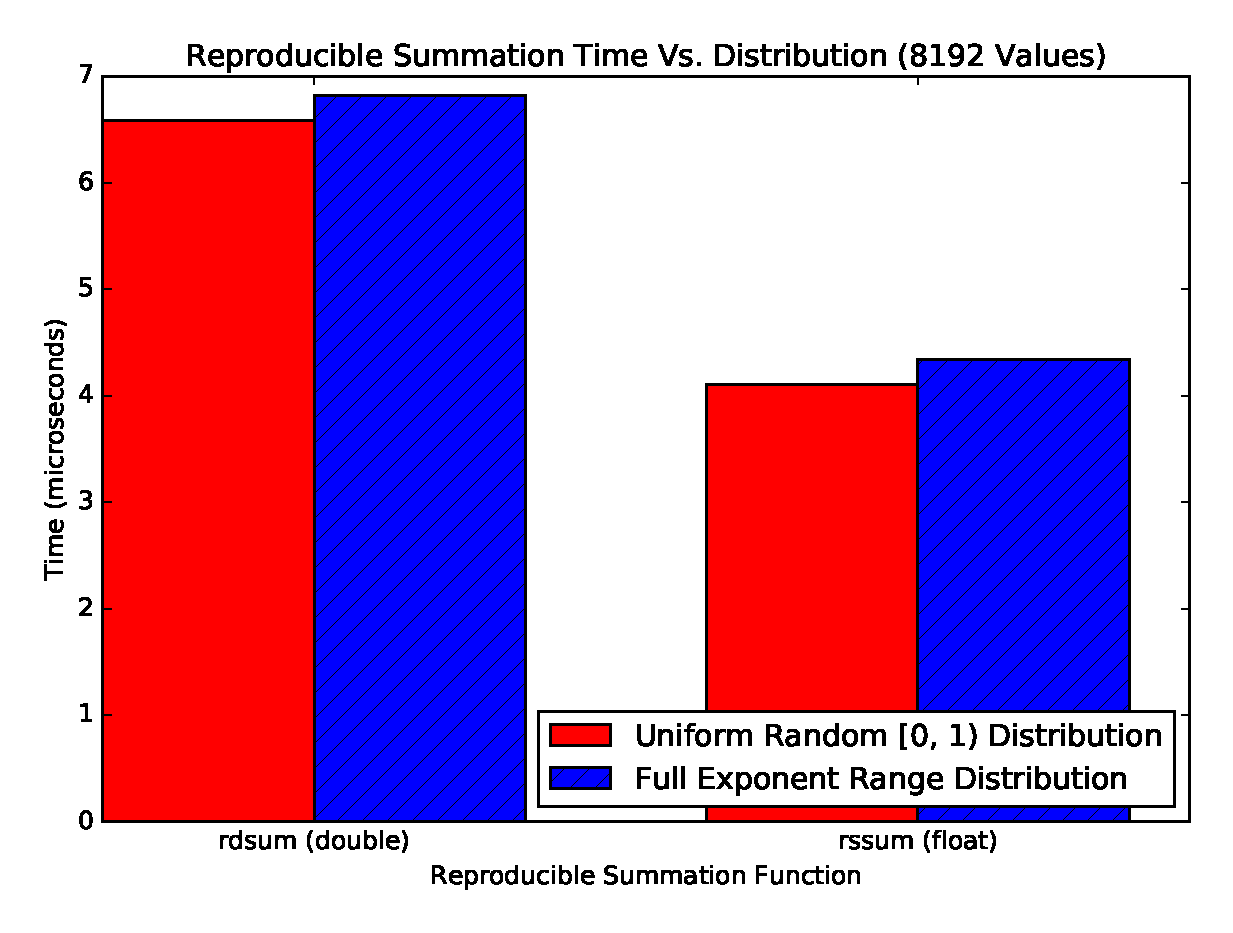
\includegraphics[width=\textwidth]{plots/easy_vs_hard}
  \caption{Time taken to sum $2^{14}$ floating point numbers of varying difficulty.}
  \label{fig:easy_vs_hard_timings}
  \end{center}
  \end{figure}
  \subsubsection{BLAS1}

    We show how our reproducible summation stacks up against a simple $C$ \texttt{for}-loop in Figure \ref{fig:forloop_timings}. Time (measured relative to the peak theoretical time for recursive summation) is shown for each method. The double-precision floating point numbers to be summed are normally distributed with mean $0$ and variance $1$. For several good reasons (lack of vectorization, lack of loop unrolling, etc.) the \texttt{for}-loop is not running at peak. With this in mind, reproducible summation is competitive with a simple \texttt{for}-loop.
  \begin{figure}[H]
  \begin{center}
  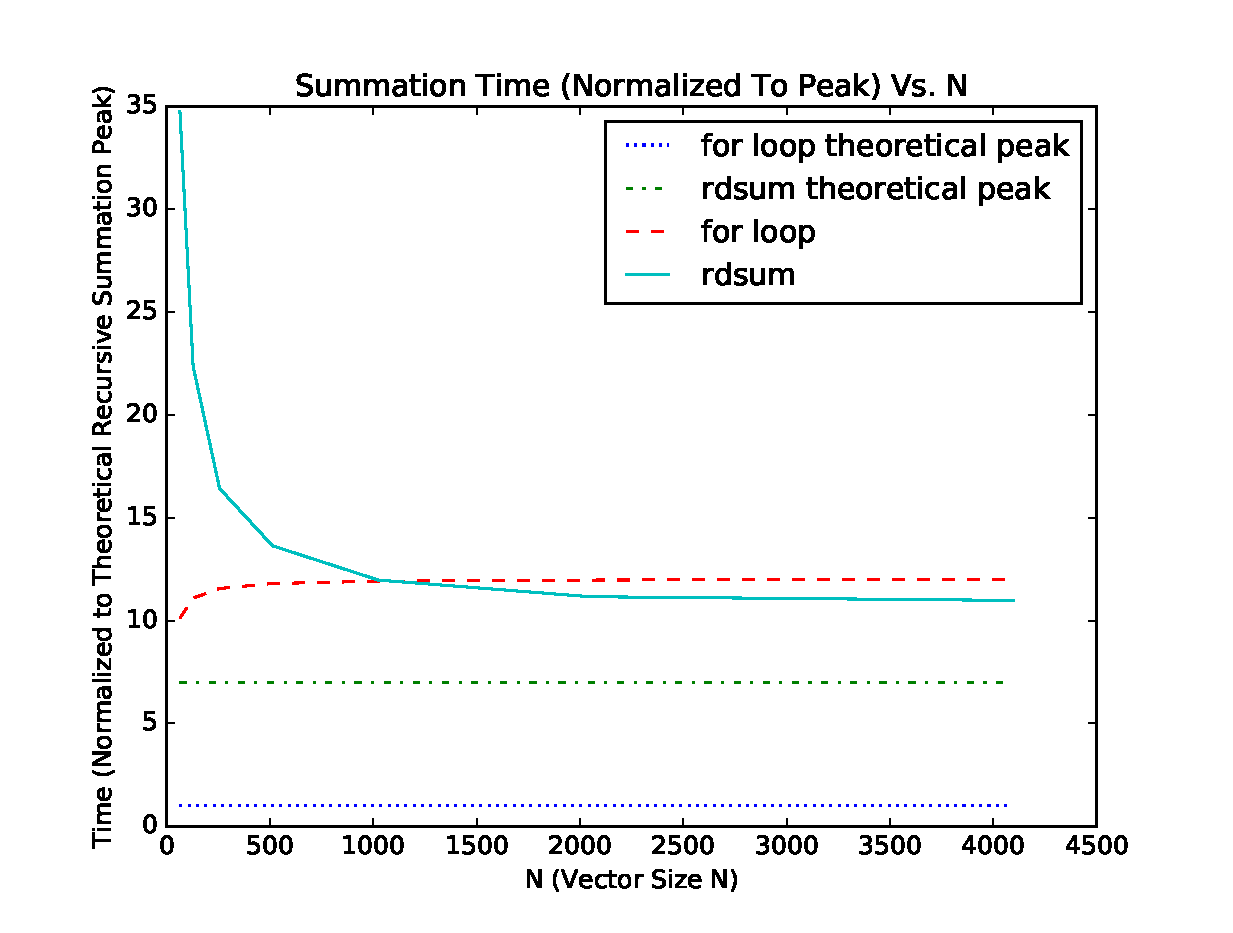
\includegraphics[width=\textwidth]{plots/sum_comparison}
  \caption{Relative floating point summation time}
  \label{fig:forloop_timings}
  \end{center}
  \end{figure}
    To give a comparison to a BLAS1 function, we show in Figure \ref{fig:dot_timings} timings of the reproducible dot product versus the MKL BLAS dot product. Again, the double-precision floating point data is distributed such that the products of the two input vectors are normally distributed with mean $0$ and variance $1$.
  \begin{figure}[H]
  \begin{center}
  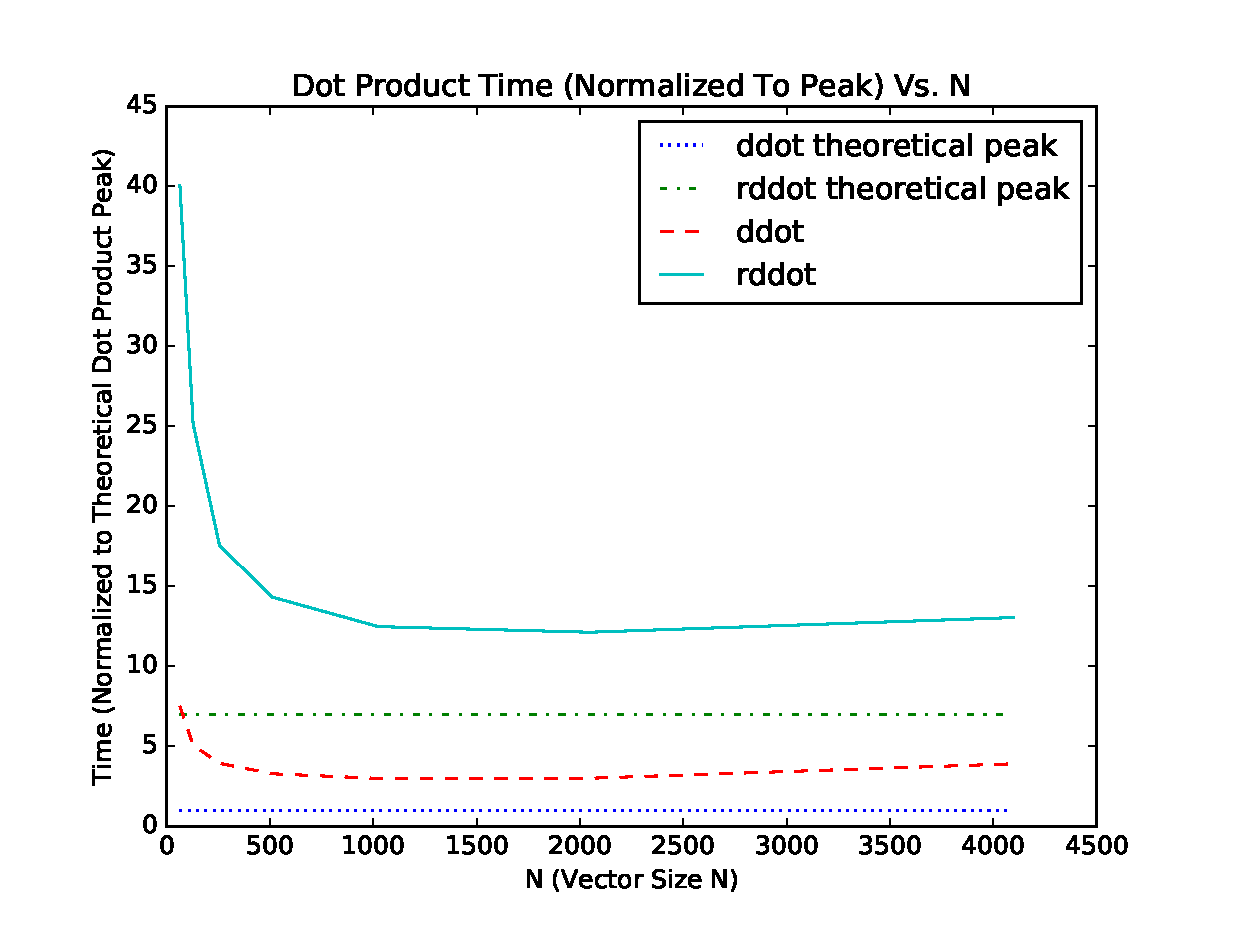
\includegraphics[width=\textwidth]{plots/dot_comparison}
  \caption{Relative dot product time}
  \label{fig:dot_timings}
  \end{center}
  \end{figure}
  \subsubsection{BLAS2}
    We show in Figure \ref{fig:gemv_timings} timings of the reproducible matrix-vector product versus the MKL BLAS matrix-vector product. The double-precision floating point data is distributed such that the products of elements of the input vector and elements of the matrix are normally distributed with mean $0$ and variance $1$.
  \begin{figure}[H]
  \begin{center}
  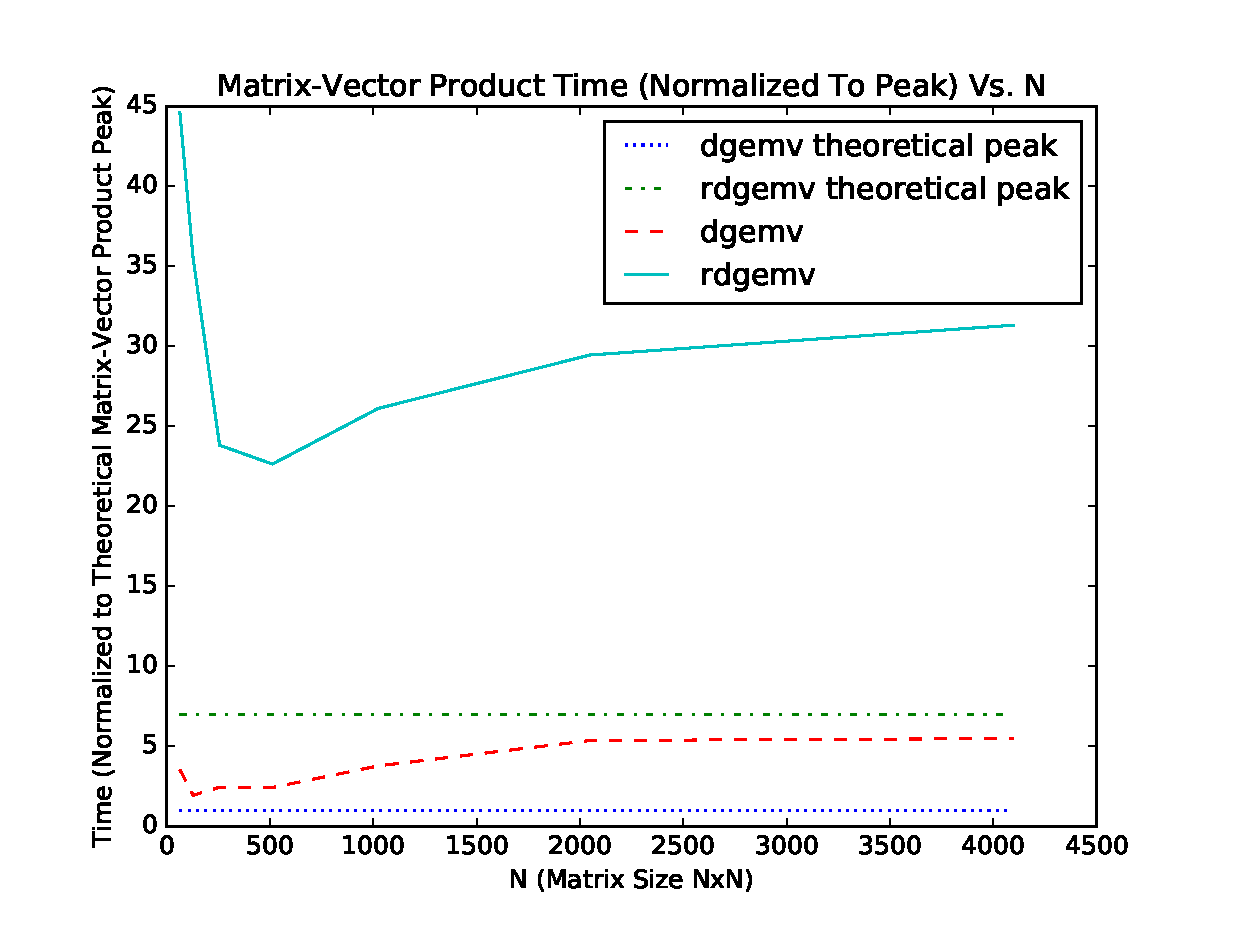
\includegraphics[width=\textwidth]{plots/gemv_comparison}
  \caption{Relative matrix-vector product time}
  \label{fig:gemv_timings}
  \end{center}
  \end{figure}
  The non-transposed matrix-vector product is the only case where composition of BLAS2 and BLAS3 functions did not achieve close to optimal results. Because the reproducible dot product operates most efficiently on contiguous sections of memory, the matrix must be transposed so that memory can be read contiguously. This causes the reproducible matrix-vector product to perform poorly due to the extra cost of matrix transposition in an already memory-bound routine. In future versions of the library, this method could be improved by writing a custom inner-loop kernel that does not make calls to \texttt{xixdot}. The kernel would operate on the primary fields of several indexed types at the same time using vectorized operations.

  The transposed matrix-vector product performs better than the non-transposed case. Timings are shown in Figure \ref{fig:gemv_trans_timings}. The reader should notice that in this case, the reproducible routine is only about a factor of two times slower than the optimized BLAS routine.
  \begin{figure}[H]
  \begin{center}
  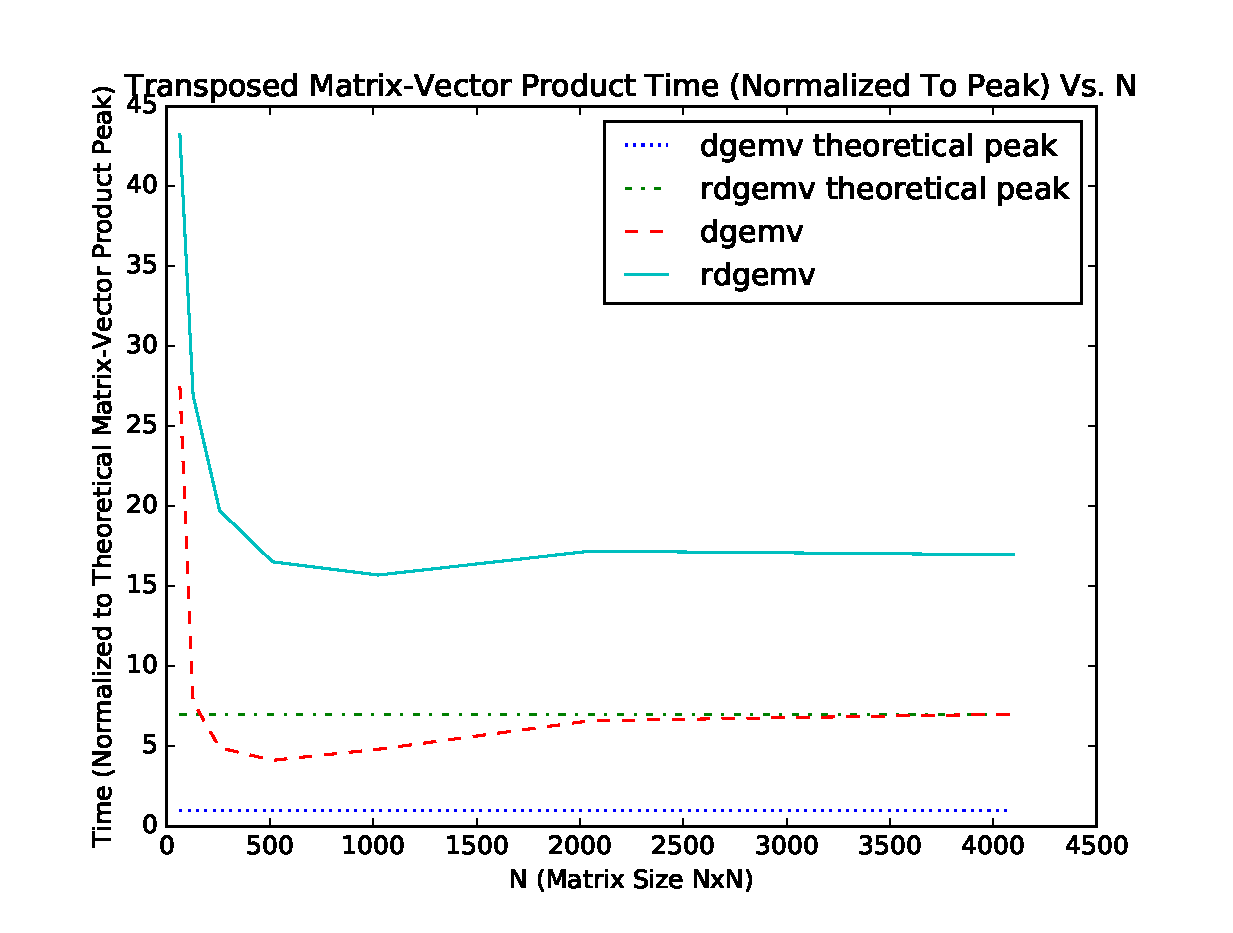
\includegraphics[width=\textwidth]{plots/gemv_trans_comparison}
  \caption{Relative transposed matrix-vector product time}
  \label{fig:gemv_trans_timings}
  \end{center}
  \end{figure}

  \subsubsection{BLAS3}
    We show in Figure \ref{fig:gemm_timings} timings of the reproducible matrix-matrix product versus the MKL BLAS matrix-matrix product. The double-precision floating point data is distributed such that the products of elements of one input matrix and the other are normally distributed with mean $0$ and variance $1$. Because the timings for each transposition case (transposing or not transposing $A$ or $B$) are similar, we show only the standard case for brevity. In this case, since both routines are running close to peak, the reproducible routine is about a factor of 8 times slower than the optimized BLAS routine.
  \begin{figure}[H]
  \begin{center}
  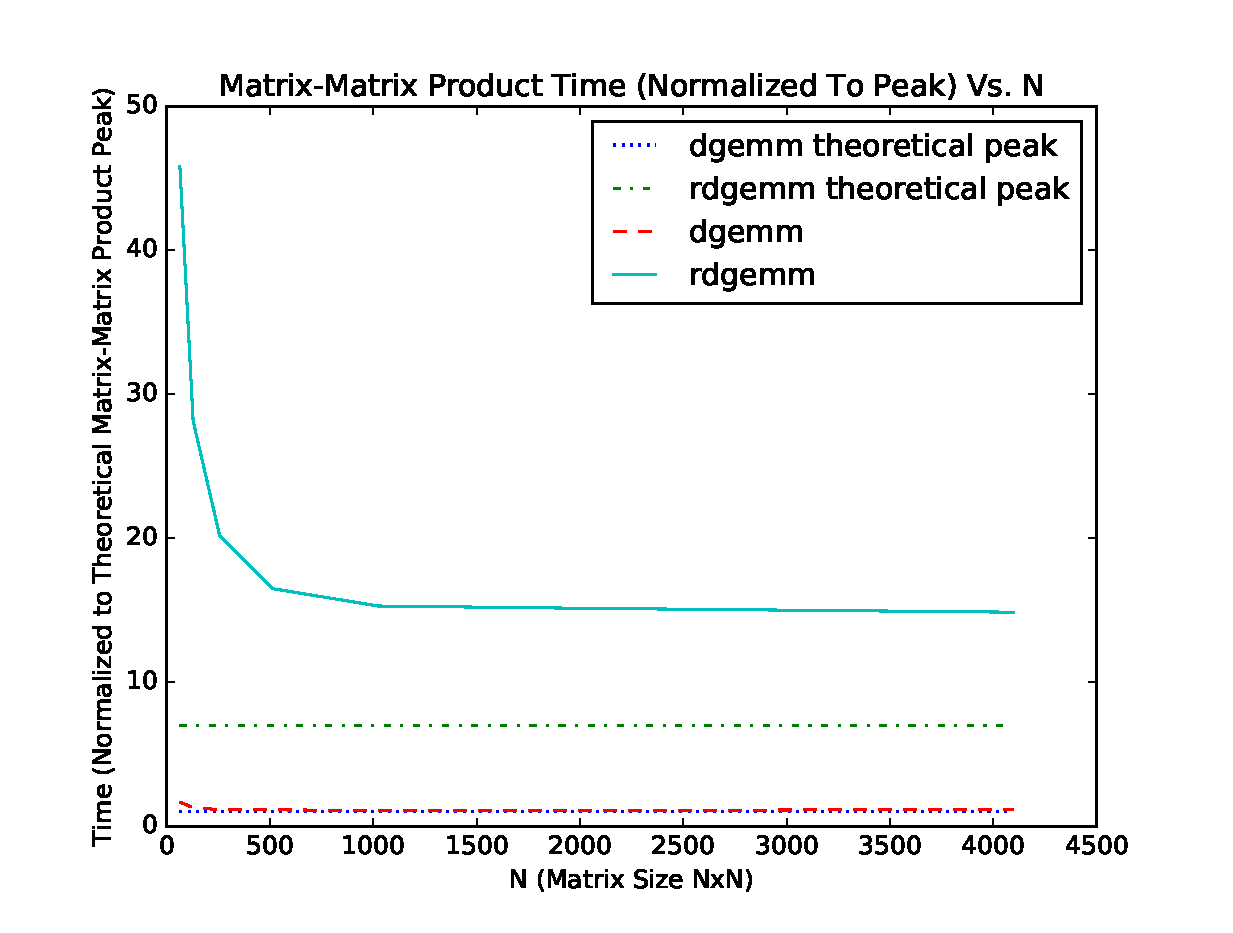
\includegraphics[width=\textwidth]{plots/gemm_comparison}
  \caption{Relative matrix-matrix product time}
  \label{fig:gemm_timings}
  \end{center}
  \end{figure}
